%!TEX root = ../template.tex
\typeout{NT FILE chapter-proposed-solution.tex}%



% ===================================================================
\chapter{Proposed Work}
\label{ch:proposed-work}
% ===================================================================
 
\section{Problem Framing and Research Questions}
\label{sec:pw-problem-rq}
 
Chapter~\ref{ch:related-work} closed by identifying four gaps that recur
across the literature on heritage AR: a technical gap around large,
continuous, multi-POI tracking; an experiential gap around connecting a
historical surface to its later and present states; an engagement gap
around sustaining attention across a content-dense surface; and a
personalisation gap that the evidence in \S\ref{subsec:rw-personalisation}
suggests is disproportionately under-served relative to its measured
impact. We treat these four gaps as defining the problem this thesis
addresses, and frame the resulting research questions at the level of a
\emph{heritage wall}, not one specific installation. The Grande
Panorama de Lisboa remains our central motivating case throughout, but
nothing below depends on its particulars; where a design decision is
genuinely specific to one surface, we say so explicitly.
 
One framing decision deserves stating before the questions
themselves: our initial intention was to treat large-scale tracking as
an open technical problem requiring a built and validated solution.
Having since tested and selected an existing visual positioning service
(\S\ref{sec:pw-techstack}), this thesis's technical contribution is
better described as configuring and empirically evaluating an existing
tool for a surface class it has not previously been validated against,
instead of inventing tracking from first principles. That is a narrower but
real contribution, since Design Science Research treats a
configured artefact and its evaluation as a legitimate unit of
contribution distinct from the underlying algorithm \cite{hevner2004}.
 
\paragraph{Central research question.} How can a mobile AR framework, built
around an existing visual positioning service, provide stable multi-POI
spatial registration, historically layered content, and visitor-adaptive
personalisation across large-scale heritage wall surfaces — and what
engagement, usability, and learning outcomes does such a framework produce
for real visitors?
 
This central question decomposes into five sub-questions, each scoped to
something our planned evaluation (\S\ref{sec:pw-evaluation}) can actually
speak to:
 
\begin{description}
  \item[\textbf{RQ1 --- Tracking configuration.} ] How should an
  off-the-shelf visual positioning service be mapped and configured to
  sustain stable, multi-POI registration across heritage walls that differ
  in geometry (planar, U-shaped, or curved) and in lighting stability
  (controlled indoor versus variable outdoor)?
 
  \item[\textbf{RQ2 --- Scalability and legibility.}] What level-of-detail
  and clustering strategy keeps a mobile AR interface legible and
  performant when a single wall carries on the order of a hundred or more
  points of interest?
 
  \item[\textbf{RQ3 --- Engagement patterns.}] What patterns of dwell time,
  point-of-interest selection, and circuit completion emerge from real,
  voluntary visitor use of the application, and how do these patterns vary
  with content structure such as circuit length or visitor profile?
 
  \item[\textbf{RQ4 --- Personalisation effectiveness.}] Does adapting
  content depth and route suggestions to a small set of self-reported
  visitor profiles produce a measurable difference in satisfaction or
  engagement relative to non-adapted content?
 
  \item[\textbf{RQ5 --- Immediate knowledge gain.}] Does a single AR-guided
  session produce a measurable, self-reported gain in historical knowledge
  about the depicted period, relative to a brief pre-session baseline?
\end{description}
 
Several questions from earlier drafts of this work are left out on purpose
(longitudinal knowledge retention over one to two weeks, a controlled AR-versus-no-AR between-subjects comparison, and psychophysiological measurement of presence), not because they lack
merit, but because none of them is answerable with the in-situ analytics,
exit survey, and short follow-up questionnaire this thesis's evaluation
plan can realistically support (\S\ref{sec:pw-evaluation}). Each returns
as future work in the closing chapter; none is listed here
as a question this thesis claims to answer. Table~\ref{tab:rq-method-map}
summarises how each retained question connects back to a related-work
finding and forward to a specific evaluation method.
 
\begin{table}[h]
\centering
\caption{Each research question traced from its motivating gap to the
method that will evaluate it.}
\label{tab:rq-method-map}
\small
\begin{tabular}{p{1.1cm}p{4.5cm}p{2.6cm}p{4.4cm}}
\toprule
\textbf{RQ} & \textbf{Motivating gap (Ch.~2)} & \textbf{Addressed in} & \textbf{Evaluated via} \\
\midrule
RQ1 & Technical gap, \S\ref{subsec:rw-large-scale} & \S\ref{sec:pw-techstack} & Field tracking tests \\
RQ2 & Technical gap, \S\ref{subsec:rw-gap} & \S\ref{sec:pw-app-concept} & Performance profiling \\
RQ3 & Engagement gap, \S\ref{subsec:rw-visitor-models} & \S\ref{sec:pw-app-concept} & In-app analytics \\
RQ4 & Personalisation gap, \S\ref{subsec:rw-personalisation} & \S\ref{sec:pw-app-concept} & Analytics + exit survey \\
RQ5 & Experiential gap, \S\ref{subsec:rw-evaluation} & \S\ref{sec:pw-app-concept} & Pre/post knowledge check \\
\bottomrule
\end{tabular}
\end{table}
 
 
\section{Domain and Case Study Context}
\label{sec:pw-domain}

This thesis's case-study choices were not fixed in advance; each follows
from a limitation the previous one exposed, and each contributes
something the other two cannot. The Grande Panorama de Lisboa motivated
the project but is closed to the public; Chafariz Velho filled that gap
and, being structurally harder, first suggested that a single
wall-specific application would not generalise; a third wall, the Alto
de Santa Catarina mural, was added to test that suggestion directly. The
three are introduced below, each with its specific role, before
Figure~\ref{fig:walls-combined} sets them side by side.

\subsection{The Grande Panorama de Lisboa --- The Motivating Case}
\label{subsec:pw-panorama}
 
The Grande Panorama de Lisboa is a 23-metre azulejo tile panel attributed,
on stylistic grounds, to Gabriel del Barco (c.~1648--1703) and generally
dated to around 1700 \cite{gacpanorama,baroqueartpanorama}. It depicts
roughly 14\,km of the Tagus waterfront across more than 150 identifiable
structures \cite{gacpanorama}, and survives as the single most complete
pictorial record of Lisbon \emph{before} the 1755 earthquake, which
destroyed most of what it depicts. It is catalogued as item no.~1 at the
Museu Nacional do Azulejo (MNAz) \cite{fcshpanorama}, Lisbon's
most-visited national museum in 2024 \cite{observador2025mnaz}. Its
value here is stakes, not convenience: no other candidate wall
carries the same density of content or public visibility. That same
value is what makes its closure since 1 November 2025 for PRR-funded
renovation, with no confirmed reopening date \cite{publico2025prr}, so
costly: it is why the Panorama could not serve as this thesis's
development surface.
 
\subsection{Chafariz Velho de Pa\c{c}o de Arcos --- The Development Case}
\label{subsec:pw-chafariz}
 
Chafariz Velho is a large, free-standing Pombaline-era fountain at
Pa\c{c}o de Arcos, Oeiras, with sources disagreeing on its exact
construction date (1755 or 1775) and its blue-and-white tilework added
considerably later, in the 1950s \cite{oeirasallabout2026,oeiraschafarizes2026}.
Its value here is access combined with difficulty: being permanently and
publicly accessible, it is where every tracking test and development
milestone in Chapters~\ref{ch:proposed-work}--\ref{ch:work-plan}
actually happens, and it is also the harder surface class: circular,
not U-shaped, so it additionally requires yaw tracking on top of the
depth coordinate the Panorama demands
(\S\ref{subsec:rw-ar-concepts-tracking}), and it sits outdoors under shifting
natural light instead of MNAz's controlled gallery lighting. A
framework proven against the harder of two cases is the stronger claim.
Chafariz Velho anchors the tracking and
architecture decisions later in this chapter.

\subsection{The Alto de Santa Catarina Mural --- The Generalisability Case}
\label{subsec:pw-generalisability}

Two cases sharing a tiled surface and a Pombaline-era connection cannot
alone support a claim of generalisability: both remain azulejo
heritage walls depicting built Lisbon. A third case breaks that
similarity. The Alto de Santa Catarina mural, in Linda-a-Velha (Oeiras),
is an outdoor urban-art wall painted by Tiago Hacke, unveiled in 2023,
depicting local wildlife, not architecture
\cite{newinoeiras2023mural}. Its value here is to stress-test the framework's assumptions. Its
geometry is angled, not curved (two planar faces at roughly 120°, wrapping the corner of the reservoir it is painted on, still requiring yaw tracking across the join); its subject is not historical but contemporary; and,
most importantly, it has no equivalent of the other walls' ``fate since an
event'' axis. A painted heron has no earthquake status, and content here
is organised by species, not building category. If a wall can
legitimately have \emph{no} status dimension, that property cannot be a
fixed field the system always expects, which is why, from
\S\ref{sec:pw-app-concept} onward, both the category and status axes are
treated as wall-supplied data, never as framework-level assumptions.

\begin{figure}[h]
\centering
\includegraphics[width=0.98\textwidth]{5-Figures/my_figures/wall_images_combined.png}
\caption{The three case-study walls used throughout this thesis, left to
right: a) Grande Panorama de Lisboa (MNAz), the central motivating case;
b) Chafariz Velho de Pa\c{c}o de Arcos, the primary development
and tracking-test surface; c) Alto de Santa Catarina mural,
Linda-a-Velha, the generalisability test case.}
\label{fig:walls-combined}
\end{figure}

The property that matters most architecturally is status: the Panorama's
earthquake fate and Chafariz's own, unrelated status marker both have
something to show, while the mural has \emph{no} status dimension at
all, so that property can never be a fixed field the system always
expects. A full property-by-property comparison of the three walls
(length, geometry, setting, content type, status axis, and access) is
given in Appendix~\ref{app:case-comparison}. Design decisions in the
remainder of this chapter are tested against the hardest applicable case
for each property (geometry against Chafariz Velho, taxonomy flexibility against the mural) so the resulting framework does not
depend on any single wall's geometry, content type, or access conditions
to function.















% ===================================================================
\section{Research Approach}
\label{sec:pw-approach}
% ===================================================================
 
This thesis follows \textbf{Design Science Research (DSR)}, which treats
the construction and rigorous evaluation of an IT artefact as a
legitimate contribution provided it addresses a genuine class of
problems, not one organisation's specific need
\cite{hevner2004}. That matches how the research questions in
\S\ref{sec:pw-problem-rq} are framed around heritage walls generally, not
the Grande Panorama specifically. Two further traditions sharpen this
default in ways DSR alone does not. Since evaluation happens with real
visitors at a real heritage site,
\textbf{Design-Based Research (DBR)}'s emphasis on generalisable design
principles developed inside uncontrolled, real-world settings describes
our evaluation context more precisely
\cite{wanghannafin2005,andersonshattuck2012}. And since early hands-on
testing of tracking approaches on Chafariz Velho
(\S\ref{subsec:pw-chafariz}) sharpened our understanding of which
research questions were answerable before those questions were
finalised, \textbf{Research-through-Design (RtD)}'s argument that problem
framing and design exploration typically co-evolve, instead of
proceeding in strict linear order \cite{zimmerman2007}, describes how
this project actually unfolded better than a clean DSR narrative would on
its own. In short: DSR justifies treating the artefact itself as a
contribution, DBR justifies evaluating it in an uncontrolled real-world
setting, and RtD justifies the order in which this thesis's own problem
framing and design work actually happened.
 
In practice, these three traditions converge on a single operating
cycle for this thesis: \emph{analyse, design, implement, evaluate,
refine}, repeated across successive iterations instead of executed once.
Figure~\ref{fig:dbr-cycle} shows this cycle. Analysis draws on
Chapter~\ref{ch:related-work} and on direct testing against our two case
surfaces; design and implementation produce a working increment of the
TileStories application (\S\ref{sec:pw-app-concept}); evaluation combines
the formative and summative methods described below; and refinement
feeds findings back into the next iteration's analysis. Feature
prioritisation within each iteration follows MoSCoW (Must/Should/Could/
Won't), weighed against visitor value, technical feasibility, and
relevance to the research questions in \S\ref{sec:pw-problem-rq}. It is a
simple enough scheme, but one that imposes a useful discipline: no
should-have feature begins development before the current iteration's
must-have features are working and evaluated.
 
\begin{figure}[h]
\centering
\resizebox{0.62\textwidth}{!}{%
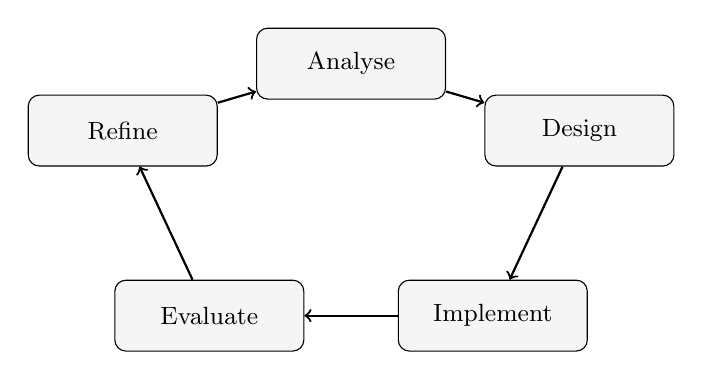
\begin{tikzpicture}[
  every node/.style={font=\fontsize{9}{11}\selectfont},
  box/.style={draw, rounded corners, align=center, minimum width=2.4cm, minimum height=0.9cm, fill=gray!8}
]
  \node[box] (analyse) at (0,1.7) {Analyse};
  \node[box] (design) at (2.9,0.85) {Design};
  \node[box] (implement) at (1.8,-1.5) {Implement};
  \node[box] (evaluate) at (-1.8,-1.5) {Evaluate};
  \node[box] (refine) at (-2.9,0.85) {Refine};
 
  \draw[->, thick] (analyse) -- (design);
  \draw[->, thick] (design) -- (implement);
  \draw[->, thick] (implement) -- (evaluate);
  \draw[->, thick] (evaluate) -- (refine);
  \draw[->, thick] (refine) -- (analyse);
\end{tikzpicture}%
}
\caption{The iterative analyse-design-implement-evaluate-refine cycle followed across development iterations, after Wang \& Hannafin's DBR model \cite{wanghannafin2005} and Hevner et al.'s DSR build-evaluate loop \cite{hevner2004}.}
\label{fig:dbr-cycle}
\end{figure}
 
Evaluation itself runs at two distinct levels of formality, and keeping
them separate matters for how each is reported later in this thesis.
\emph{Formative} evaluation happens at the end of each development
iteration: short, task-based sessions with five to eight participants,
using a think-aloud protocol so that moment-to-moment confusion,
misread affordances, and unexpected navigation choices surface while they
are still cheap to fix \cite{nielsen1994}. This sample size is
intentionally small — Nielsen's heuristic-evaluation tradition treats five
participants as sufficient to surface most usability problems in a single
round, and at this stage we are hunting for breakages, not measuring
effect sizes. \emph{Summative} evaluation, described fully in
\S\ref{sec:pw-evaluation}, happens once near the end of development and
is held to a different standard: it is the evidence base for RQ3 through
RQ5, drawing on in-app analytics, a short exit survey, and where feasible
a brief follow-up, collected primarily at Chafariz Velho given the access
constraints discussed in \S\ref{subsec:pw-panorama}, with deployment at
MNAz pursued opportunistically if the museum reopens before submission.
 
This two-level structure is also where DSR's and DBR's slightly different
priorities resolve cleanly instead of conflicting: DSR asks whether the
artefact works and generalises; DBR asks what we learned about designing
for this class of setting regardless of whether one specific deployment
succeeds outright. Each iteration's refinement step is meant to report
both, not collapse them into a single pass/fail judgement of the app.



















% ===================================================================
\section{App Concept: TileStories}
\label{sec:pw-app-concept}
% ===================================================================
 
\subsection{Core Concept and Key UX Decisions}
\label{subsec:pw-core-concept}
 
TileStories takes its name from the medium and the method at once: tiles,
the physical azulejo surface, and stories, the narratives a visitor
unlocks by interacting with it. The core proposition is simple (point a phone at the wall and the city it depicts comes alive) but holding
to it consistently shapes every decision below. Architecturally,
TileStories is better understood as a config-driven framework than a
single fixed application: each wall's points of interest, categories,
and content are authored as structured data consumed by a small, reusable
set of content renderers, closer to a headless CMS than a bespoke app
rebuilt per installation. This is what makes the three-wall
generalisability claim of \S\ref{subsec:pw-generalisability} buildable,
not just aspirational: a fourth wall is added by writing data, not by
rewriting renderers. Figure~\ref{fig:logo} shows the visual identity,
finalised early and, as \S\ref{sec:wp-completed} notes, independently of
the later Flutter-to-Unity change.

\begin{figure}[h]
\centering

\includegraphics[width=0.5\textwidth]{5-Figures/my_figures/app_logo.png}
\caption{TileStories visual identity.}
\label{fig:logo}
\end{figure}
 
Four UX decisions follow directly from Chapter~\ref{ch:related-work} and
recur across this feature set:

\begin{aitemize}[nosep]
\item \textbf{Free exploration by default.} 
Circuits are optional overlays; nothing forces a visitor down one path. Gkatsou found non-linear structures suit museum visitors better than fixed sequences\cite{gkatsou2018}.
\item \textbf{Progressive disclosure.} A floating label identifies a
point of interest spatially; full content opens in a fixed bottom sheet,
avoiding the information-overload risk Wang et al.\ identify in dense AR
scenes \cite{wang2025grand} --- the mechanism RQ2 asks about directly.
\item \textbf{Restrained, period-appropriate visual language.} A muted
sepia/azulejo-blue palette lets the technology mediate the artefact
instead of competing with it \cite{recupero2019}, with one exception:
colour-coded status indicators (survived/modified/destroyed) on the
timeline, where colour carries information the palette alone cannot.
\item \textbf{Camera-optional by design.} Every feature remains
available through a browse mode, for visitors who prefer not to use AR
or cannot for accessibility reasons; screen-reader support is tested
against Unity's native TalkBack/VoiceOver APIs from Phase~0, not assumed.
\end{itemize}

Together, these decisions implement what Wang and Zhu describe as a
closed interaction loop, where the physical wall anchors the experience
while POI cards, the timeline, circuits, and light gamification
(\S\ref{subsec:pw-feature-phases}) form a virtual layer that keeps
pulling the visitor back through it \cite{wangzhu2022}.
 
\subsection{Feature Set by Phase}
\label{subsec:pw-feature-phases}
 
The feature set is staged so that each phase widens scope in one
dimension at a time: first a single wall tracks reliably, then a single
point of interest is fully fleshed out, then points of interest connect
into a visit, then the working result is extracted into something
reusable, then that reusable core is proven on an unseen wall, and only
then is the whole thing frozen and measured. Table~\ref{tab:phases}
summarises the six phases plus stretch; calendar dates and the Gantt
chart are given in \S\ref{sec:wp-overview}. Light, formative testing
happens continuously within every phase (\S\ref{sec:pw-approach}), so it
is not listed as a phase of its own. Only the final, structured
in-situ evaluation is.

\begin{table}[h]
\centering
\caption{Feature set staged by phase, with each phase's primary purpose and what it tests.}
\label{tab:phases}
\small
\resizebox{\textwidth}{!}{%
\begin{tabular}{p{2.3cm}p{2.6cm}p{7.2cm}p{2.2cm}}
\toprule
\textbf{Phase} & \textbf{Focus} & \textbf{Key deliverables} & \textbf{Primarily tests} \\
\midrule
0 --- Core Tracking & Single-wall MVP & Unity/Immersal tracking pipeline (\S\ref{sec:pw-techstack}); ten hero POIs with tap-to-reveal cards; non-AR browse fallback; offline operation & RQ1 \\
1 --- POI-Level Content & One point of interest, fully realised & Full POI content model (text, image, audio narration by the guide character); onboarding into four visitor profiles with profile-adaptive depth; generalised \emph{lapse} state axis (\S\ref{sec:pw-approach}), instantiated on the Panorama as a four-epoch timeline; expansion to thirty POIs & RQ2, RQ4 \\
2 --- Scene-Level Features & Points of interest connected into a visit & Thematic circuits linking POIs; light gamification (discovery badges, short knowledge check); coverage to roughly sixty POIs & RQ3 \\
3 --- Framework Packaging & Extracting the reusable core & Core separated into a standalone Unity package; lightweight editor tool for wall configuration; Chafariz Velho re-integrated using only the packaged tooling as an internal sanity check & Generalisability (internal) \\
4 --- Template \& Third-Wall Validation & Proving generalisation on an unseen wall & Core packaged as an installable Unity project template; Alto de Santa Catarina mural integrated using only that template --- this integration doubles as the time-to-new-wall protocol of \S\ref{sec:pw-evaluation} & Generalisability (external) \\
5 --- Evaluation Readiness & Freeze and measure & Full analytics instrumentation; exit survey; pre/post knowledge check; English translation; structured in-situ evaluation sessions; no new features added & RQ1--RQ5 \\
5+ --- Stretch (time-permitting) & Additional, not required & GPT-based conversational guide layered alongside the scripted narrative; animated earthquake sequence; 360° interior views; Spanish/French localisation & --- \\
\bottomrule
\end{tabular}
}
\end{table}

A diagram tracing the main paths through the application (onboarding, AR scanning and lock, and the timeline and circuit branches that sit alongside free exploration) is provided in
Appendix~\ref{app:prototypes} alongside the screen-level UI prototypes;
none of these paths is unconventional enough for an app of this kind to
warrant detailed discussion in the body.

% ===================================================================
\section{Technology Stack: Comparison, Tests, and Decisions}
\label{sec:pw-techstack}
% ===================================================================
 
This thesis's tracking and frontend decisions evolved across two distinct
phases: an initial desk-based comparison of available options, followed
by hands-on implementation and testing that overturned part of that
initial comparison. Both phases are reported here, since the reversal
itself is informative: a theoretical technology comparison, however
careful, can reach a confident wrong answer that only hands-on testing
exposes. The account below is tidier in
hindsight than the decision felt at the time. In practice there was a fair amount of back-and-forth between the two frontend
options before the Immersal test results made the tracking choice obvious.
 
\subsection*{Tracking: From a Hand-Built System to a Visual Positioning Service}
 
Four tracking approaches were evaluated for registering content against a
large, continuous heritage wall: a hand-built anchor-plus-world-coordinate
system layered on top of ARFoundation's native image tracking; Vuforia
Image Targets; Vuforia Area Targets; and Immersal, a photogrammetry-based
visual positioning service (VPS). Wang and Zhu's taxonomy of mobile AR
tracking (marker-based, natural-feature-based, and hybrid approaches \cite{wangzhu2022}) places the first two options in the natural-feature
category and the latter two in approaches that build a persistent spatial
model of the environment instead of tracking a single reference image.
 
The hand-built system was implemented first and tested extensively,
including on Chafariz Velho. It detects one or more printed reference
images via ARFoundation and computes a wall-local coordinate frame from
whichever images are currently visible, re-aligning that frame as
additional images come into view. Testing surfaced a specific and
informative failure mode: when two reference images disagree slightly on
the wall's pose (an unavoidable consequence of measurement error and ARCore's own pose noise) the system enters a visible ``ping-pong,''
repeatedly correcting position back and forth as different images take
priority. Eliminating this required successively more elaborate
filtering, ending in a momentum-based smoothing scheme; a Kalman filter
would be the theoretically principled choice for this kind of fixed-target
noise problem and is flagged as a stronger future alternative to the
heuristic actually implemented \cite{kingmaba2015}. The broader lesson
generalises beyond this one implementation: a hand-built multi-anchor
system can be made workable, but only by re-deriving, ad hoc and
imperfectly, the persistent spatial modelling a dedicated VPS provides
natively.
 
Vuforia Area Targets were rejected for a more basic reason: generating
an area target requires a full 3D geometric scan of the surface,
officially supported only via LiDAR-equipped Apple hardware, Matterport
cameras, or professional terrestrial scanners, none of which a
researcher, or most museums, can be assumed to have access to. Commercial
licensing also requires Vuforia's Premium tier, priced on request and
estimated in industry discussion at roughly \$840--1{,}500 per year. Both
constraints cut against this thesis's generalisability goal: a tracking
approach tied to specific Apple hardware or an undisclosed enterprise
licence does not scale easily to a new heritage wall.
 
Immersal, by contrast, builds its spatial model from ordinary photographs
captured with any AR-capable smartphone, processed through
structure-from-motion photogrammetry into a point-cloud map that can be
localised either via the cloud or, for offline-first deployment, fully
on-device once downloaded. A recent controlled comparison evaluating
Vuforia, Immersal, MultiSet, and the ARCore Geospatial API found both
Vuforia and Immersal achieved indoor positioning errors generally below
4\,cm \cite{skabek2026}; the same study found Immersal more robust to
severe lighting reduction, while Vuforia proved more robust against
certain high-contrast structured visual noise. Neither dominates
unconditionally, but our own device testing supports a clear conclusion
on the dimension that matters most here: an Immersal integration, built
against the official Unity SDK, localised successfully against a test map
in two to three seconds on a real Android device, with all test points of
interest spawning at their correct positions.
 
Table~\ref{tab:tracking-matrix} sets out the resulting decision across
nine weighted criteria. The weights themselves reflect this thesis's
specific priorities: hardware accessibility and ease of mapping a new
wall are weighted heavily because both follow directly from the
generalisability goal stated throughout this chapter, not because they
are universally the most important AR-tracking criteria in general.
 
\begin{table}[h]
\centering
\caption{Weighted comparison of the four tracking approaches evaluated.
Scores (1--10) reflect this project's own testing combined with vendor
documentation and the comparative literature cited above, not an
independent third-party benchmark.}
\label{tab:tracking-matrix}
\small
\resizebox{\textwidth}{!}{%
\begin{tabular}{p{7.0cm}p{0.9cm}p{1.1cm}p{1.2cm}p{1.1cm}p{1.2cm}}
\toprule
\textbf{Criterion} & \textbf{Wt.} & \textbf{Custom} & \textbf{Vuforia Img.} & \textbf{Vuforia Area} & \textbf{Immersal} \\
\midrule
Hardware accessibility (no LiDAR/scanner) & 9 & 10 & 10 & 2 & 10 \\
Re-localises without a specific anchor in view & 8 & 2 & 2 & 10 & 10 \\
Accuracy/drift over a 20--40\,m wall & 8 & 4 & 6 & 9 & 8 \\
Robust to occlusion (visitors passing through) & 8 & 5 & 5 & 9 & 9 \\
Generalisable to mapping a \emph{new} wall quickly & 7 & 4 & 6 & 3 & 9 \\
Initialisation/first-lock speed & 6 & 7 & 7 & 8 & 8 \\
Offline/on-device capable & 6 & 10 & 10 & 8 & 9 \\
App size overhead & 4 & 10 & 7 & 3 & 7 \\
Commercial licensing cost & 5 & 10 & 9 & 5 & 6 \\
\midrule
\textbf{Weighted total (max 610)} & & \textbf{398} & \textbf{411} & \textbf{396} & \textbf{529} \\
\bottomrule
\end{tabular}
}
\end{table}
 
Immersal's advantage in Table~\ref{tab:tracking-matrix} is driven
primarily by the two criteria most specific to this thesis's framing:
hardware accessibility and new-wall generalisability. It is not driven
by dominating every row. This is, in fact, the honest version of the
``compare two systems and that becomes the contribution'' idea raised
during early problem framing (\S\ref{sec:pw-problem-rq}): the comparison
was real and is reported here, but the contribution it supports is a
configuration decision, not a head-to-head system built specifically to
be benchmarked. \textbf{Immersal is the tracking approach used for the
remainder of this thesis.}
 
\subsection*{Frontend: Unity over Flutter}
 
The frontend decision does not follow automatically from the tracking
decision, and is worth justifying separately. Flutter offers markedly
better tooling for the UI-heavy parts of this application (onboarding, content cards, circuits, surveys) and an early framework comparison,
conducted before tracking tests began, scored Flutter ahead of Unity
overall for that reason. What that comparison could not anticipate is
that Immersal's officially supported integration is Unity-native, with
AR Foundation and ARCore/ARKit already wired in; reaching the same
integration from Flutter would mean maintaining a native AR rendering
layer, including camera-to-screen projection mathematics a game engine
normally handles automatically, on two platforms. Given that reliable
large-scale tracking is this thesis's primary technical risk (RQ1), and
Unity's weaker UI tooling a real but lower-stakes cost by comparison,
this thesis builds in Unity end-to-end. The features initially assumed
to require Flutter are all implementable in Unity's UI Toolkit; the
interface will need more deliberate design attention to avoid feeling
game-like, but no feature in \S\ref{sec:pw-app-concept} depends on a
capability Unity lacks.
 
\subsection*{Data and Backend: A Deliberately Brief Decision}
 
Unlike tracking and frontend, the data architecture for this thesis is a
conventional choice that does not warrant extended justification: point-
of-interest content (text, image paths, audio paths, epoch and category
metadata) is stored locally and bundled with the application, guaranteeing
full offline operation regardless of museum or outdoor connectivity,
while anonymous usage analytics (the events instrumented from \S\ref{sec:pw-app-concept}'s Phase~5 onward) are logged to a managed
backend service for later analysis. 




% ===================================================================
\section{System Architecture Overview}
\label{sec:pw-architecture}
% ===================================================================
 
This thesis adopts a narrow, on-purpose split between two layers: a
\emph{Core} layer holding infrastructure that behaves identically
regardless of which heritage wall is loaded, and a \emph{Walls} layer
holding one self-contained folder per installation, so that adding a
future wall means adding a new folder without modifying shared logic.
This mirrors the generalisability argument at the code level
(\S\ref{subsec:pw-generalisability}). Deciding what belongs in Core
followed a conservative rule: something moves in only once a second wall
needs it unchanged, following Fowler's Rule of Three \cite{fowler1999}.
Four systems cleared that bar early (AR session bootstrap, POI/timeline UI, analytics and survey pipeline, and the guide character and audio player) while everything else (POI datasets, geometry
parameters, circuit definitions) stays inside each wall's own folder as
data, intentionally allowed to differ between walls without a shared
interface forcing a common shape. Per Sandi Metz's argument that a wrong
shared abstraction costs more to unwind than tolerated duplication
\cite{metz2016}, two similar-looking wall folders are cheaper to keep
separate than an abstraction that turns out not to fit a future wall's
geometry.

Each wall is described by a single Unity ScriptableObject holding its
Immersal map identifier, POI dataset reference, and basic metadata; its
content is packaged as its own Addressables group, Unity's recommended
mechanism for on-demand content \cite{unityaddressables2026}, keeping the
base application small as more walls are added. Figure~\ref{fig:architecture}
shows the resulting structure: the camera feed is localised by Immersal,
the returned pose lets Core place that wall's POIs, and the resulting
interaction is logged through Core's analytics regardless of which wall
produced it. The three case-study walls of
\S\ref{subsec:pw-generalisability} occupy this diagram directly: each is its own \texttt{Walls/} folder running the
same Core unmodified, which is the concrete, testable form the
generalisability claim takes at the architecture level, and what makes
packaging the Core as a reusable Unity template
(\S\ref{sec:wp-overview}) a natural extension of the design, not
an afterthought.

\begin{figure}[h]
\centering
\resizebox{\textwidth}{!}{%
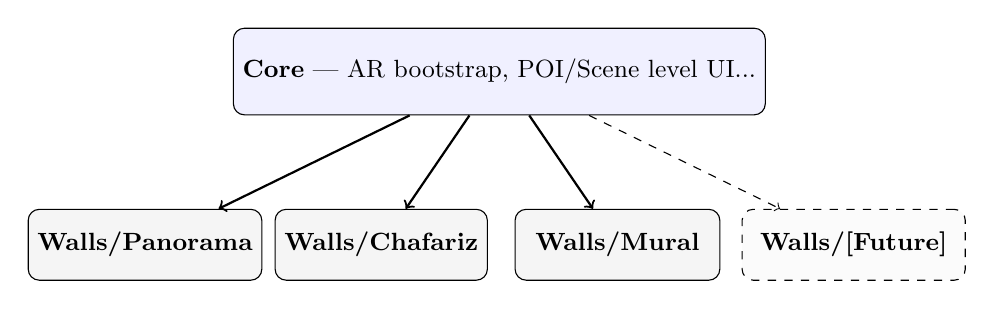
\begin{tikzpicture}[
  every node/.style={font=\fontsize{9}{11}\selectfont},
  core/.style={draw, rounded corners, align=center, minimum width=5cm, minimum height=1.1cm, fill=blue!6},
  wall/.style={draw, rounded corners, align=center, minimum width=2.6cm, minimum height=0.9cm, fill=gray!8},
  future/.style={draw, dashed, rounded corners, align=center, text width=2.6cm, minimum height=0.9cm, fill=gray!3}
]
  \node[core] (core) at (0,0) {\textbf{Core} --- AR bootstrap, POI/Scene level UI...};
  \node[wall] (panorama) at (-4.5,-2.2) {\textbf{Walls/Panorama}};
  \node[wall] (chafariz) at (-1.5,-2.2) {\textbf{Walls/Chafariz}};
  \node[wall] (mural) at (1.5,-2.2) {\textbf{Walls/Mural}};
  \node[future] (future) at (4.5,-2.2) {\textbf{Walls/[Future]}};
 
  \draw[->, thick] (core) -- (panorama);
  \draw[->, thick] (core) -- (chafariz);
  \draw[->, thick] (core) -- (mural);
  \draw[->, dashed] (core) -- (future);
\end{tikzpicture}%
}
\caption{Core/Walls architecture: shared infrastructure stays minimal; each of the three case-study walls is an independent, addressable content package, with any future wall following the same pattern.}
\label{fig:architecture}
\end{figure}















% ===================================================================
\section{Evaluation Plan}
\label{sec:pw-evaluation}
% ===================================================================
 
Evaluating a heritage AR application properly is harder than the
literature sometimes implies. Chatsiopoulou and Michailidis's recent
systematic review of forty-five cultural-heritage AR studies found that
evaluation approaches in this field vary considerably in rigour, and that
many applications begin an evaluation process without completing it
thoroughly \cite{chatsiopoulou2025}. We take this as licence to state
scope plainly instead of overreaching: the plan below distinguishes
what this thesis can guarantee from what depends on circumstances outside
its control, and is sized to what a single researcher can realistically
execute within a six-month development window.
 
\subsection{Research Design}
\label{subsec:pw-research-design}
 
The evaluation runs across two tracks. The \emph{guaranteed track} takes
place at Chafariz Velho, permanently and freely accessible, recruiting
participants directly from passersby on the Pa\c{c}o de Arcos seafront.
It follows a single-condition, in-situ design (participants use the application freely for a short, unguided session) consistent with
both how most studies in Chatsiopoulou and Michailidis's review approach
evaluation and the unguided-exploration design Bauer, Hagler, and Kocur
plan for their own large-surface mural application
\cite{chatsiopoulou2025,bauer2025}. A genuine AR-versus-no-AR comparison,
of the kind Bachiller, Monzo, and Rey conducted at a technological
heritage museum \cite{bachiller2023}, would strengthen causal claims but
needs a control group and roughly double the recruitment effort; we treat
it as a stretch addition attempted only if recruitment proves easier than
expected.

The \emph{opportunistic track} applies only if MNAz reopens with enough
time remaining for a further round of evaluation, using the same
instruments at the Grande Panorama itself to show that findings from
Chafariz Velho transfer to an indoor, higher-POI-density installation.
Nothing in this thesis's research questions or contribution claims
depends on this track completing; if it happens, it is reported as
additional evidence of generalisability.
 
\subsection{Evaluation Instruments}
\label{subsec:pw-eval-instruments}
 
Five instruments make up the core battery, chosen specifically for being
administrable by a single researcher with a street-recruited, time-
limited participant. The System Usability Scale (SUS) anchors the
quantitative usability assessment: ten items, five to ten minutes to
complete, and benchmarked against widely-used interpretive thresholds
(below 51 poor, 51--68 acceptable, above 68 good) that let a single
session's results be compared against published norms without needing a
control group of our own \cite{brooke1996,bangor2008}. Sauter et al.\
report SUS scores in the good range (broadly 70s to low 80s) across two
evaluation cycles of their own mobile AR heritage-photo application,
which gives a directly comparable benchmark for a structurally similar
system \cite{sauter2024}. The Short User Experience Questionnaire
(UEQ-S) complements SUS with eight items covering pragmatic quality
(efficiency, clarity) and hedonic quality (stimulation, novelty),
dimensions SUS does not capture and that matter specifically for an
experience meant to feel engaging, not merely usable. The
short form is used here on purpose over the full 26-item UEQ, since a
street-recruited participant's patience is a genuinely scarce resource here.
 
A brief exit survey (five items: overall satisfaction, perceived
historical understanding, favourite feature, open-ended difficulties, and
a single recommend-to-a-friend item) and a short, single-session
historical knowledge check, administered immediately before and after
the AR session, cover RQ5's interest in immediate learning gain
(\S\ref{sec:pw-problem-rq}). We do not attempt to validate this knowledge
check as a psychometric instrument in its own right. Doing so properly,
the way Cheng et al.\ validate a seven-construct model with 266
respondents \cite{cheng2025}, needs a sample size this evaluation will not
reach, and claiming that level of rigour without the numbers to support
it would be the wrong kind of overreach. Where time and willing
participants allow, a short semi-structured conversation, modelled on
Cesário and Nisi's interview protocol with teenage and family museum
visitors \cite{cesarionisi2023} and on Souropetsis and Kyza's use of
paired interviews to reduce the social pressure of one-on-one questioning
\cite{souropetsis2025}, adds qualitative depth that a Likert scale alone
cannot. Finally, in-app analytics, instrumented from Phase~5 onward
(\S\ref{subsec:pw-feature-phases}), log dwell time, POI selection, and
circuit completion passively, giving RQ3 and RQ4 a behavioural data
source that does not depend on a participant's willingness to fill out
another form.

A sixth instrument targets the framework claim itself, not any
single RQ: a \emph{time-to-new-wall} protocol, in which one of the three
case-study walls is reintegrated from a clean project using only the
packaged framework and its documentation, with no source access and no
prior familiarity assumed. Wall-clock time to three fixed milestones (first
successful localisation, first tappable marker, first working circuit)
and every point of friction encountered are logged and reported directly.
This is not a statistical measurement but a single-run small-N: its value is in making the ``easy to add a new wall''
claim a reported number instead of an assertion, which no amount of
qualitative description of the architecture alone can substitute for.
Table~\ref{tab:eval-instruments} summarises how each instrument maps to
setting and realistic sample size.
 
\begin{table}[h]
\centering
\caption{Evaluation instruments, what they inform, and the realistic
setting and sample size for each.}
\label{tab:eval-instruments}
\small
\resizebox{\textwidth}{!}{%
\begin{tabular}{p{3.1cm}p{4.6cm}p{4.1cm}p{1.7cm}}
\toprule
\textbf{Instrument} & \textbf{Primarily informs} & \textbf{Setting} & \textbf{Realistic N} \\
\midrule
SUS & Usability (RQ1, RQ2) & Chafariz (guaranteed) & 20--30 \\
UEQ-S & Hedonic experience (RQ3) & Chafariz (guaranteed) & 20--30 \\
Exit survey & Satisfaction, profile fit (RQ4) & Chafariz (guaranteed) & 20--30 \\
Pre/post knowledge check & Immediate learning (RQ5) & Chafariz (guaranteed) & 15--25 \\
Semi-structured interview & Qualitative depth (all RQs) & Chafariz (time-permitting) & 5--10 \\
In-app analytics & Engagement patterns (RQ3, RQ4) & Both tracks & All sessions \\
Time-to-new-wall protocol & Generalisability (framework claim) & Clean project, packaged tooling only & 1 run \\
\bottomrule
\end{tabular}
}
\end{table}
 
\subsection{Ethical Considerations}
\label{subsec:pw-ethics}
 
Verbal informed consent, confirmed again before any recording, is the
minimum standard for street-recruited sessions; no personally identifying
information is collected, and analytics events use an anonymous session
identifier only. Recruiting families for the children's profile
additionally requires a parent or guardian's consent and the child's own
separately sought assent. The university's specific approval process for
this scale of study remains to be confirmed before data collection
begins.